\documentclass[border=10pt]{standalone}
\usepackage{tikz}
\usetikzlibrary{shapes.geometric, arrows.meta, positioning}

\begin{document}
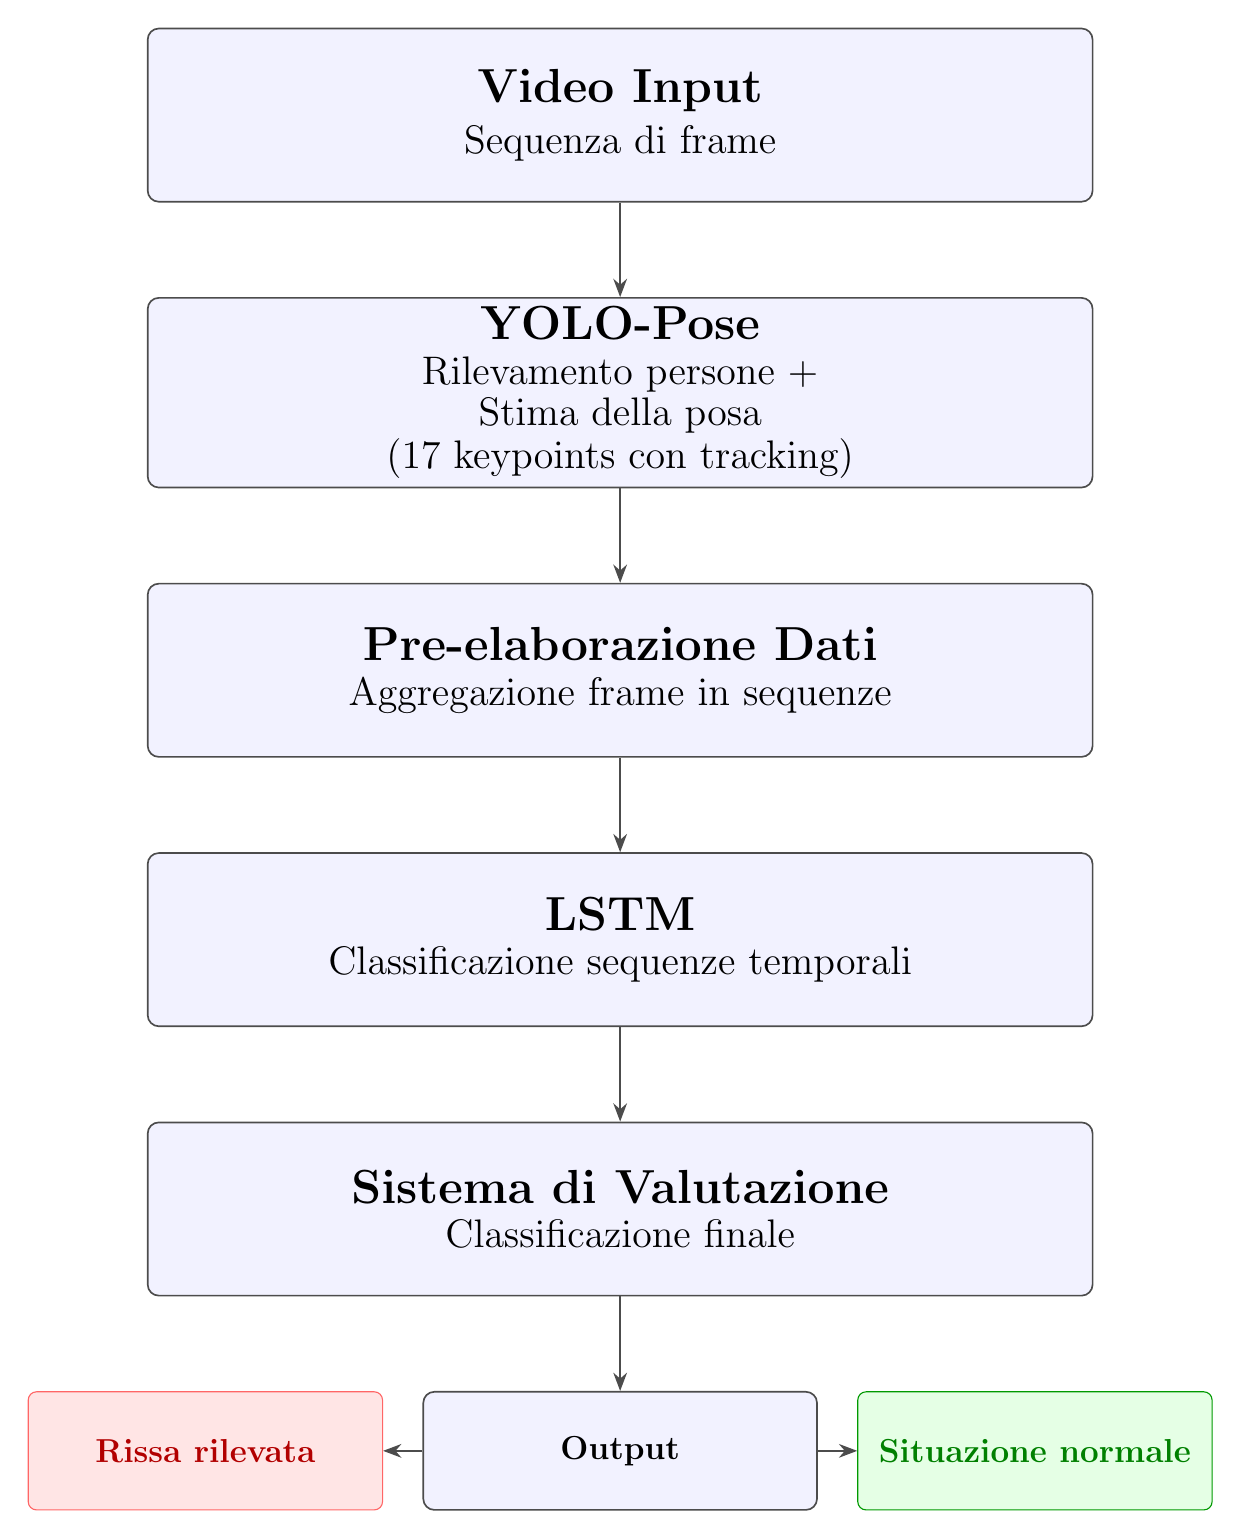
\begin{tikzpicture}[
    block wide/.style={
        rectangle, 
        draw=black!70, 
        fill=blue!5, 
        rounded corners=4pt, 
        minimum width=12cm,
        minimum height=2.2cm,
        align=center, 
        line width=0.6pt
    },
    output label/.style={
        rectangle, 
        draw=black!70, 
        fill=blue!5, 
        rounded corners=4pt, 
        minimum width=5cm,
        minimum height=1.5cm, 
        align=center, 
        font=\large\bfseries,
        line width=0.6pt
    },
    fight/.style={
        rectangle, 
        draw=red!60, 
        fill=red!10, 
        rounded corners=3pt, 
        minimum width=4.5cm, 
        minimum height=1.5cm, 
        font=\large\bfseries, 
        text=red!70!black
    },
    normal/.style={
        rectangle, 
        draw=green!60!black, 
        fill=green!10, 
        rounded corners=3pt, 
        minimum width=4.5cm, 
        minimum height=1.5cm, 
        font=\large\bfseries, 
        text=green!50!black
    },
    arrow/.style={
        -Stealth, 
        thick, 
        black!70
    }
]

\node[block wide] (input) {
    {\LARGE\bfseries Video Input}\\[4pt]
    {\Large Sequenza di frame}
};

\node[block wide, below=1.2cm of input] (yolopose) {
    {\LARGE\bfseries YOLO-Pose}\\[4pt]
    {\Large Rilevamento persone +}\\[1pt]
    {\Large Stima della posa}\\[1pt]
    {\Large (17 keypoints con tracking)}
};

\node[block wide, below=1.2cm of yolopose] (preproc) {
    {\LARGE\bfseries Pre-elaborazione Dati}\\[4pt]
    {\Large Aggregazione frame in sequenze}
};

\node[block wide, below=1.2cm of preproc] (lstm) {
    {\LARGE\bfseries LSTM}\\[4pt]
    {\Large Classificazione sequenze temporali}
};

\node[block wide, below=1.2cm of lstm] (decision) {
    {\LARGE\bfseries Sistema di Valutazione}\\[4pt]
    {\Large Classificazione finale}
};

\node[output label, below=1.2cm of decision] (output) {Output};
\node[fight, left=0.5cm of output] (fight) {Rissa rilevata};
\node[normal, right=0.5cm of output] (norm) {Situazione normale};

\draw[arrow] (input) -- (yolopose);
\draw[arrow] (yolopose) -- (preproc);
\draw[arrow] (preproc) -- (lstm);
\draw[arrow] (lstm) -- (decision);
\draw[arrow] (decision) -- (output);
\draw[arrow] (output.west) -- (fight.east);
\draw[arrow] (output.east) -- (norm.west);

\end{tikzpicture}
\end{document}
